%%%%%%%%%%%%%%%%%%%%%%%%%%%%%%%%%%%%%%%%%
% baposter Portrait Poster
% LaTeX Template
% Version 1.0 (15/5/13)
%
% Created by:
% Brian Amberg (baposter@brian-amberg.de)
%
% This template has been downloaded from:
% http://www.LaTeXTemplates.com
%
% License:
% CC BY-NC-SA 3.0 (http://creativecommons.org/licenses/by-nc-sa/3.0/)
%
%%%%%%%%%%%%%%%%%%%%%%%%%%%%%%%%%%%%%%%%%

%----------------------------------------------------------------------------------------
%	PACKAGES AND OTHER DOCUMENT CONFIGURATIONS
%----------------------------------------------------------------------------------------

\documentclass[a0paper,portrait]{baposter}
\usepackage[brazil]{babel}
\usepackage[T1]{fontenc}
\usepackage[utf8]{inputenc}
\usepackage{multicol}
\usepackage[font=small,labelfont=bf]{caption} % Required for specifying captions to tables and figures
\usepackage{booktabs} % Horizontal rules in tables
\usepackage{relsize} % Used for making text smaller in some places
\usepackage{url}
\graphicspath{{figures/}} % Directory in which figures are stored

\definecolor{bordercol}{RGB}{40,40,40} % Border color of content boxes
\definecolor{headercol1}{RGB}{255,255,255} % Background color for the header in the content boxes (left side)
\definecolor{headercol2}{RGB}{255,255,255} % Background color for the header in the content boxes (right side)
\definecolor{headerfontcol}{RGB}{0,0,0} % Text color for the header text in the content boxes
\definecolor{boxcolor}{RGB}{255,255,255} % Background color for the content in the content boxes
\usepackage{enumitem}
\usepackage{multicol}

\setlist{noitemsep}

\begin{document}

\background{ % Set the background to an image (background.pdf)
\begin{tikzpicture}[remember picture,overlay]
\draw (current page.north west)+(-2em,2em) node[anchor=north west]
{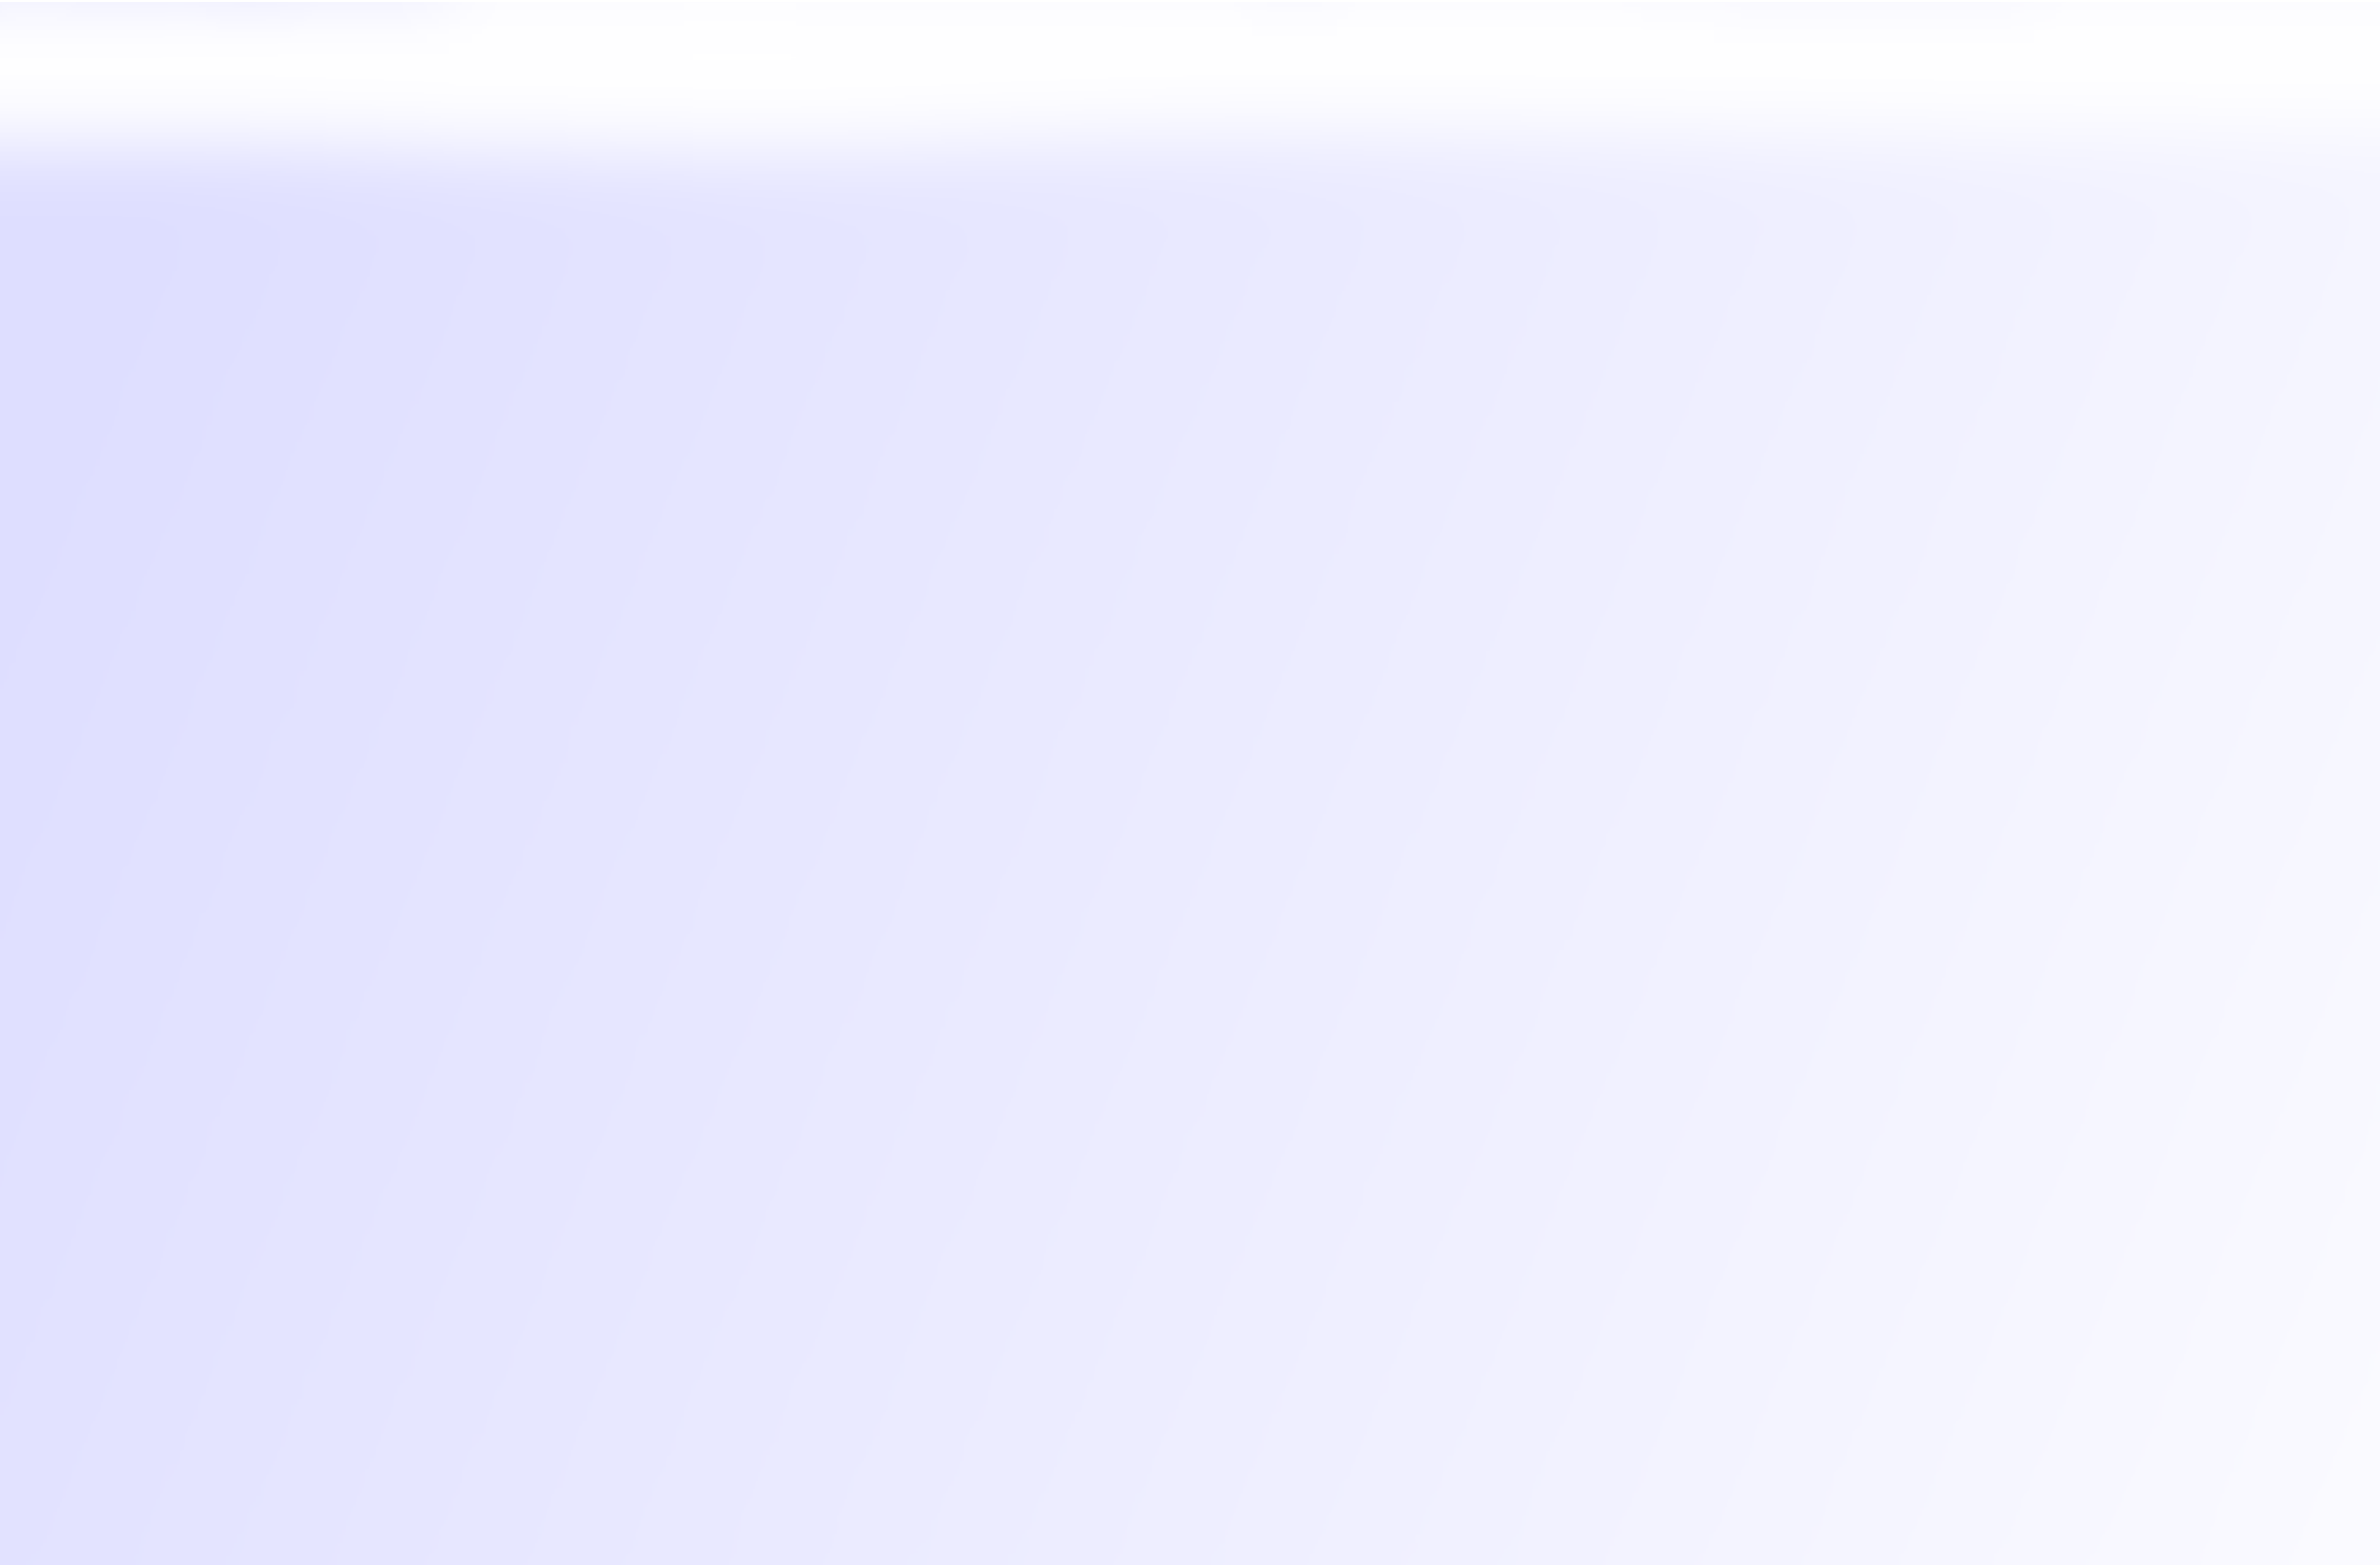
\includegraphics[height=1.1\textheight]{background}};
\end{tikzpicture}
}

\begin{poster}{
grid=false,
borderColor=bordercol, % Border color of content boxes
headerColorOne=headercol1, % Background color for the header in the content boxes (left side)
headerColorTwo=headercol2, % Background color for the header in the content boxes (right side)
headerFontColor=headerfontcol, % Text color for the header text in the content boxes
boxColorOne=boxcolor, % Background color for the content in the content boxes
headershape=roundedright, % Specify the rounded corner in the content box headers
headerfont=\Large\sf, % Font modifiers for the text in the content box headers
textborder=rectangle,
background=user,
headerborder=closed, % Change to closed for a line under the content box headers
boxshade=plain
}
{}
%
%----------------------------------------------------------------------------------------
%	TITLE AND AUTHOR NAME
%----------------------------------------------------------------------------------------
%
{\sf Explorando a Terceira Lei de Newton para \\ Simulação N-Corpos em
  uma Plataforma GPU} % Poster title
{\vspace{1em} Vinícius A. Herbstrith, Lucas Mello Schnorr\\ % Author names
{\smaller \{vaherbstrith,schnorr\}@inf.ufrgs.br}} % Author email addresses
{
\includegraphics[scale=0.10]{logo_fapergs_inf.pdf}} % University/lab logo



%----------------------------------------------------------------------------------------
%	INTRODUCTION
%----------------------------------------------------------------------------------------
\setitemize{ leftmargin=*, rightmargin=5pt}

\headerbox{Contexto}{name=introduction,column=0,row=0,span=2}{

\begin{itemize}
\item Simulações N-corpos são simulações de um sistema de partículas sobre a
influência das forças físicas externas e forças geradas pelas outras
partículas do mesmo sistema

\item Simulações deste tipo são largamente
aplicadas em astrofísica, física de plasma e dinâmica molecular

\item 
A simulação ocorre em intervalos de tempo onde, para cada intervalo e
para cada partícula, é calculada a força resultante que uma partícula
sofre devido a interação com as outras

\item Complexidade O($N^2$), onde N é a quantidade de
partículas presentes no sistema.

\item Bom desempenho no ambiente massivamente paralelo da GPU.

\item Algoritmo proposto por Halpem (CppCon2014)
\begin{itemize}
\item Terceira lei de Newton: Para toda interação, na forma de força, que um corpo A aplica sobre um corpo B, dele A irá receber uma força de mesma direção, intensidade e sentido oposto
\item Consegue reduzir o número de iterações pela metade
\item Algoritmo recursivo (evita condições de corrida)
\item Algoritmo criado com a arquitetura CPU em mente
\end{itemize}

\end{itemize}


}


%----------------------------------------------------------------------------------------
%	Objectives
%----------------------------------------------------------------------------------------

\headerbox{Objetivos}{name=objective,column=2,row=0 }{

\begin{itemize}
\item Implementação do algoritmo de Halpem em um ambiente GPGPU:
\begin{itemize}
\item  Encontrar uma alternativa para a recursão
\begin{itemize}
        \item  Recursão apresenta uma performance pobre na GPU
\end{itemize}
\item  Superar condições de corrida
\item  Definição de um novo algoritmo que se aproveite da terceira lei de Newton
\end{itemize}
\end{itemize}


}


%----------------------------------------------------------------------------------------
%	Image
%----------------------------------------------------------------------------------------

\headerbox{Simulação}{name=picture,column=2,below = objective}{ % To reduce this block to 1 column width, remove 'span=2'
\begin{center}
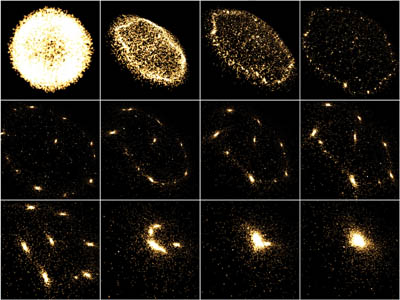
\includegraphics[width=0.85\linewidth]{gpu_sim.jpg}
\captionof{figure}{Imagem resultante da simulação executada pelo algoritmo disponibilizada em GPU Gems 3}
\end{center}
}

}

%----------------------------------------------------------------------------------------
%	Conclusion
%----------------------------------------------------------------------------------------

\headerbox{Conclusões}{name=conclusion,column=2,below = picture}{ % To reduce this block to 1 column width, remove 'span=2'
\begin{itemize}
    \item Resultado até 6 vezes inferior à uma implementação força bruta
    \item Razões
        \begin{itemize}
        \item Necessidade de Mutex
        \item Modelo mestre-trabalhador
        \item Não se paroveitar da localidade de memória
        \end{itemize}
    \item Trabalhos futuros:
        \begin{itemize}
        \item Implementação em um ambiente em cluster
        \end{itemize}
\end{itemize}

}



%----------------------------------------------------------------------------------------
%	REFERENCES
%----------------------------------------------------------------------------------------

\headerbox{Referências}{name=references,column=2,below=conclusion}{

\smaller % Reduce the font size in this block
\renewcommand{\section}[2]{\vskip 0.05em} % Get rid of the default "References" section title
\nocite{*} % Insert publications even if they are not cited in the poster

\bibliographystyle{unsrt}
\bibliography{sample} % Use sample.bib as the bibliography file
}



%----------------------------------------------------------------------------------------
%	Implementation
%----------------------------------------------------------------------------------------

\headerbox{Implementação}{name=methods,span=2,column=0,row=0,below=introduction}{
        \begin{itemize}
            \item Decomposição da execução recursiva
            \item Processar de forma ascendente
            \begin{itemize}
                \item Comecar a partir das folhas da árvore recursiva
                \item Distribuição das folhas entre os blocos de thread da GPU
                \begin{itemize}
                    \item Gera condições de corrida
                \end{itemize}
            \end{itemize}

\item Tratando a Condição de corrida:
\begin{itemize}
    \item Evitar que blocos de thread processem uma mesma partícula
    \item Modelo mestre-trabalhador
     \begin{itemize}
        \item Mestre controla o avanço dos blocos entre as folhas
        \item Mutex para a área de código que define o papel de mestre
    \end{itemize}
    \item Blocos esperam os outros blocos terminarem o processamento
\end{itemize}

        \end{itemize}



}

--------------------------------------------------------------------------------------
%	RESULTS
%----------------------------------------------------------------------------------------

\headerbox{Experimentos}{name=results2,span=2,column=0,row=0,below=methods}{ % To reduce this block to 1 column width, remove 'span=2'


\newenvironment{experimentitemize}
{ \begin{itemize}
    \setlength{\itemsep}{5pt}
    \setlength{\parskip}{5pt}
    \setlength{\parsep}{5pt}     }
{ \end{itemize}                  } 

\begin{multicols*}{2}


\begin{itemize} 
    \item Análise de desempenho:
        \begin{itemize}
        \item 1000 particulas
        \item 10 iterações
        \item 10 execuções
    \end{itemize}
    \item Comparação com a implementacação n-corpos disponibilizada em GPU Gems
    \item Utilizamos gráficos com a média e o desvio padrão das 10 execuções
    \item Plataforma experimental:
    \begin{itemize}
        \item Processador Intel i7-4770 CPU (3.40GHz)
        \item Disco rígido HDD 1TB SATA II
        \item Memória de 8GiB DIMM DDR3(1.6GHz)
    \end{itemize}

\end{itemize}



\vfill



%------------------------------------------------


%colocar legenda embaixo com:
%               theme(legend.position="bottom") +

%------------------------------------------------

\end{multicols*}
\begin{center}
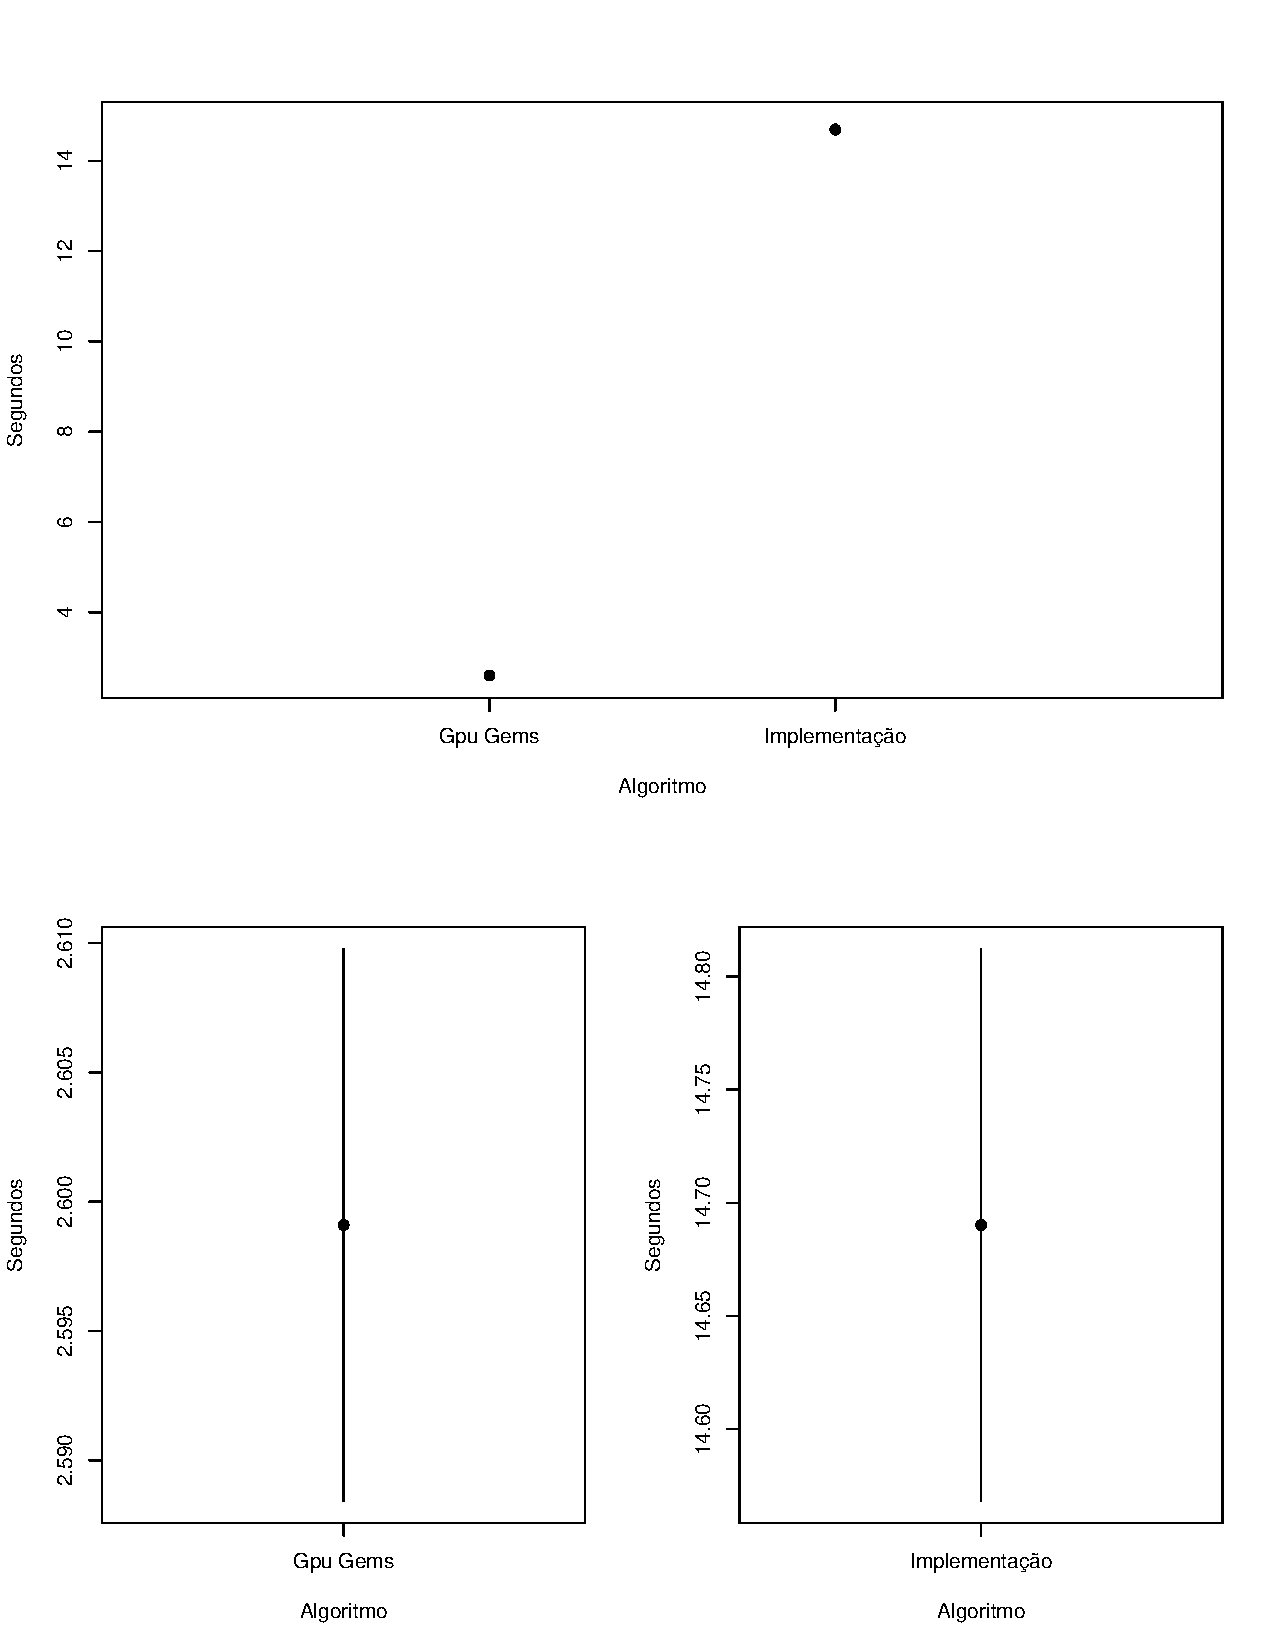
\includegraphics[width=0.45\linewidth]{avg_sd_nbody.pdf}
\captionof{figure}{Tempo de execução dos experimentos}
\end{center}
}



\end{poster}

\end{document}
